\subsection{Signup and Login}
The signup page asks to the unregistered user to provide some personal information like name, surname, email address and password. Moreover, the user has to specify if he is a student or an educator by flagging the corresponding checkbox. In case he is a student, he is also asked to provide his GitHub's username. Alternatively, users can choose to sign up using third party services like Google or GitHub.\\
\begin{figure}[H]
    \centering
    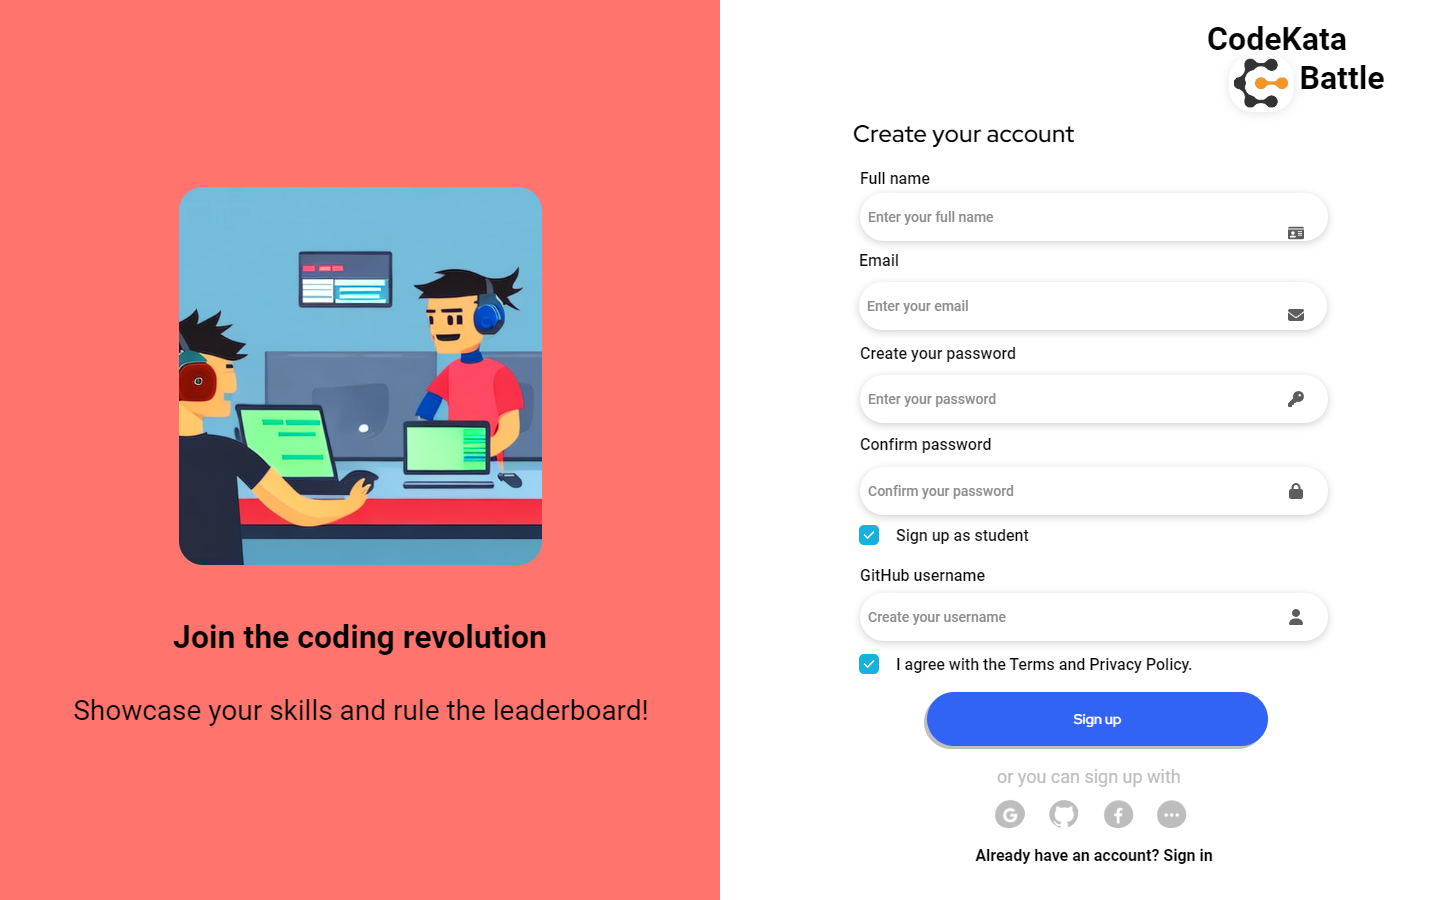
\includegraphics[width=0.8\textwidth]{Mockups/1_signup.png}
    \caption{Signup page}
\end{figure}
\newpage
The login page asks to the registered user to provide his email address and password. Alternatively, users can choose to login using the same third party services.\\
\begin{figure}[H]
    \centering
    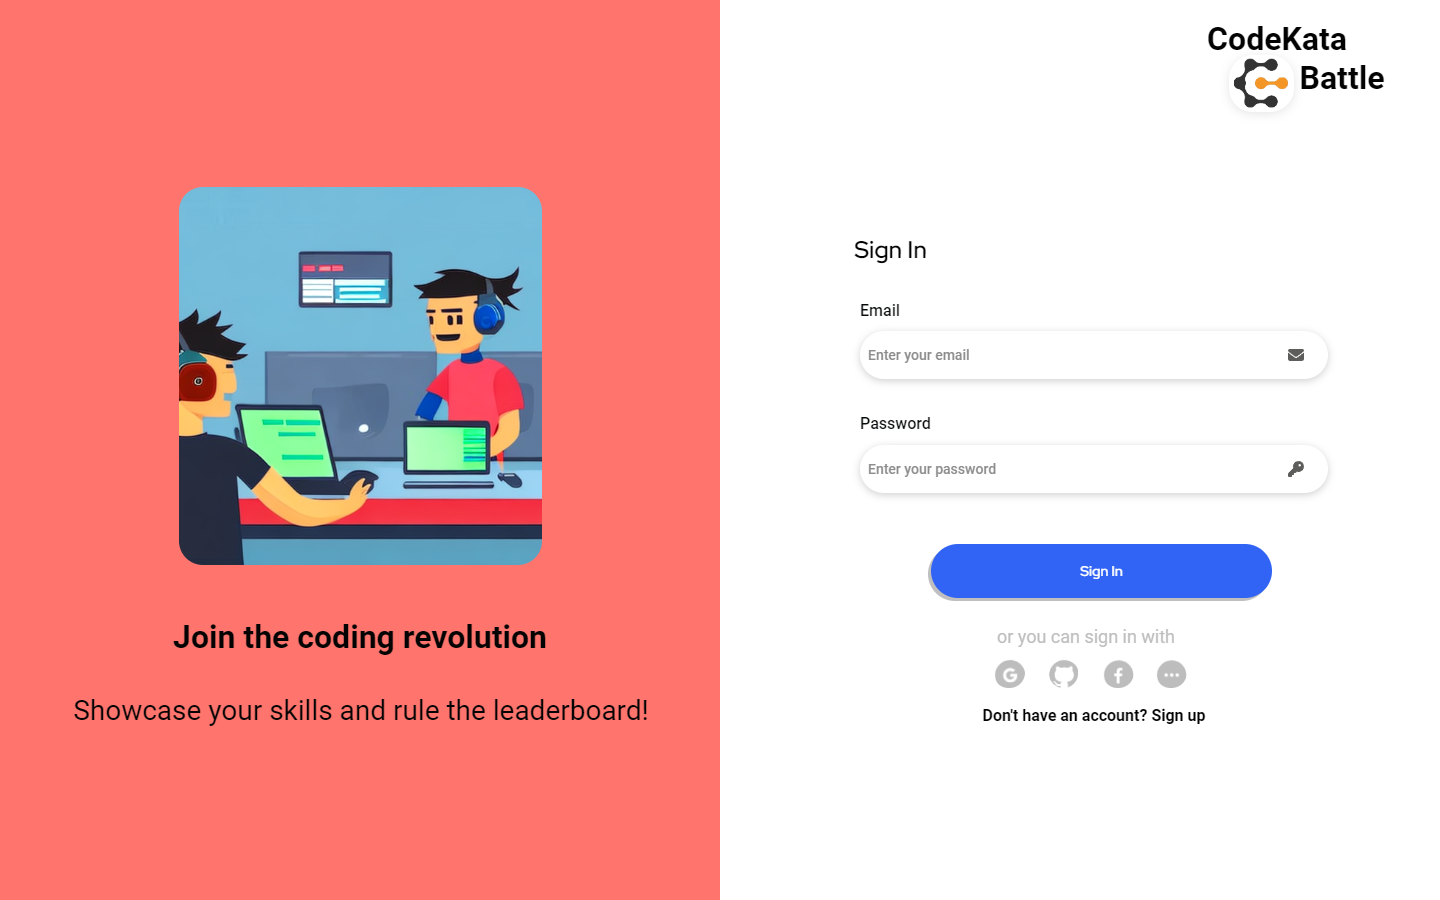
\includegraphics[width=0.8\textwidth]{Mockups/2_login.png}
    \caption{Login page}
\end{figure}

\subsection{Home page}
The home page is the first page that the user sees after logging in. If the logged user is a student, the homepage contains a brief overview of platform's ongoing tournaments, battles the user is participating in, a calendar with upcoming deadlines and some statistics of past battles. Educator's homepage is similar, but will include some information about tournaments and battles he is responsible of. \\
\begin{figure}[H]
    \centering
    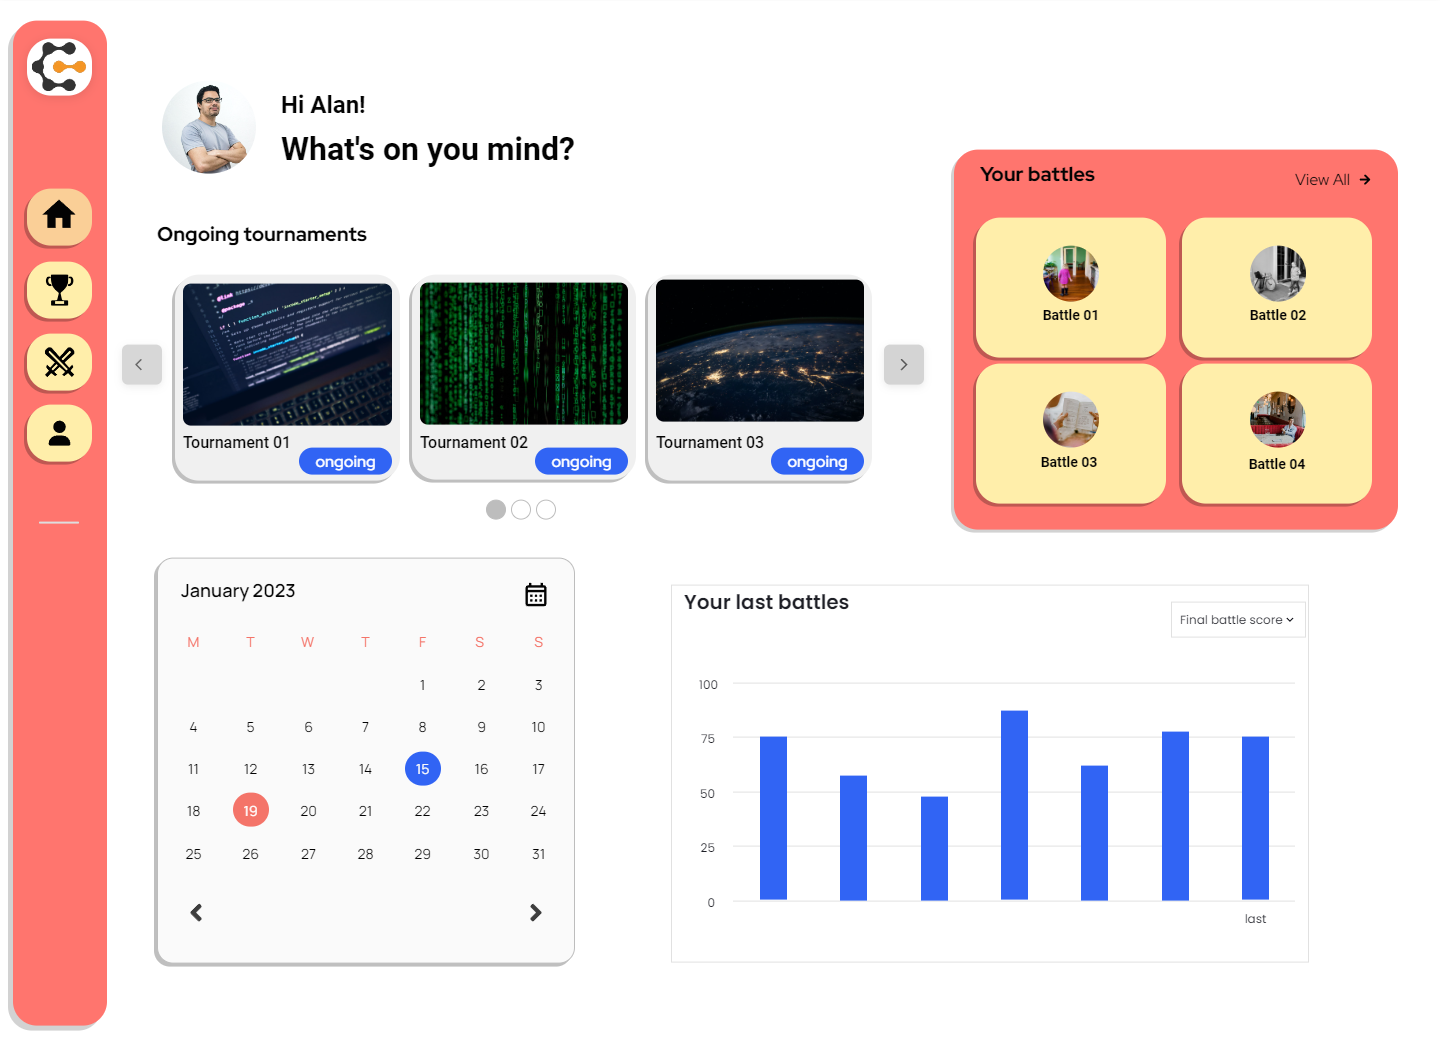
\includegraphics[width=0.8\textwidth]{Mockups/3_student_homepage.png}
    \caption{Home page from the perspective of an user logged as student}
\end{figure}

\subsection{Tournaments}
The tournaments section will provide to the student a list of all ongoing tournaments in the platform and a list with all tournaments the student is enrolled in. The page will contain also some collections, to access for example popular tournaments or all past tournaments. By clicking on a tournament, the user will be redirected to the tournament page.\\ 
\begin{figure}[H]
    \centering
    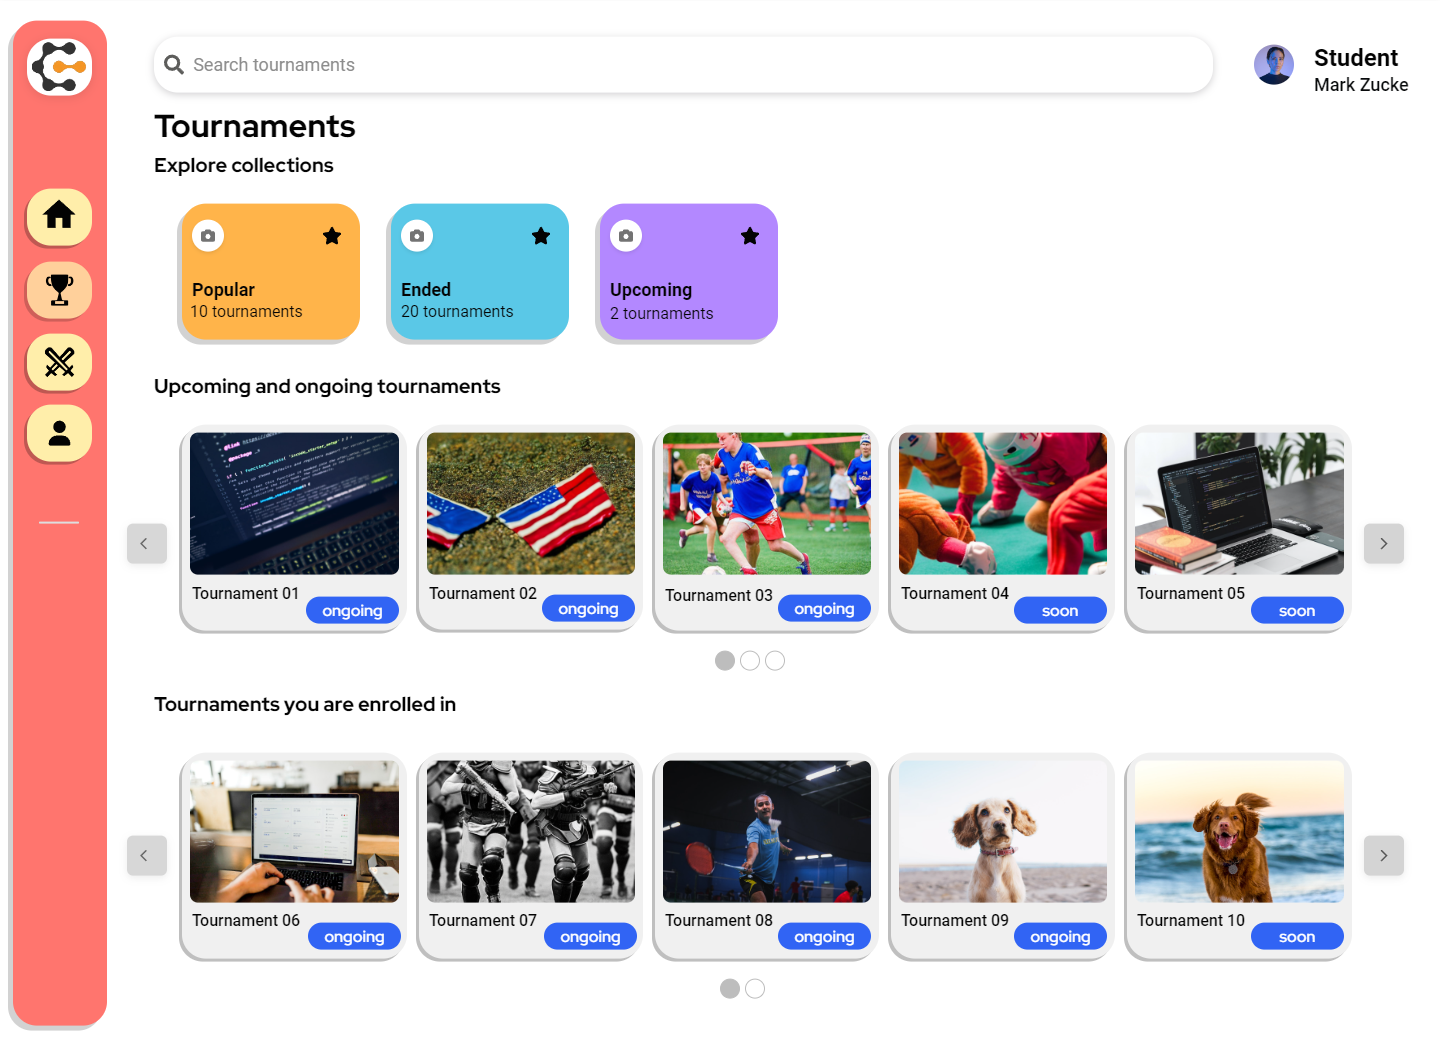
\includegraphics[width=0.8\textwidth]{Mockups/4_student_tournaments.png}
    \caption{Tournaments page from the perspective of an user logged as student}
\end{figure}
The corresponding page for educators will show basic similar information about tournaments, but will also provide a button to create a new tournament.\\
\begin{figure}[H]
    \centering
    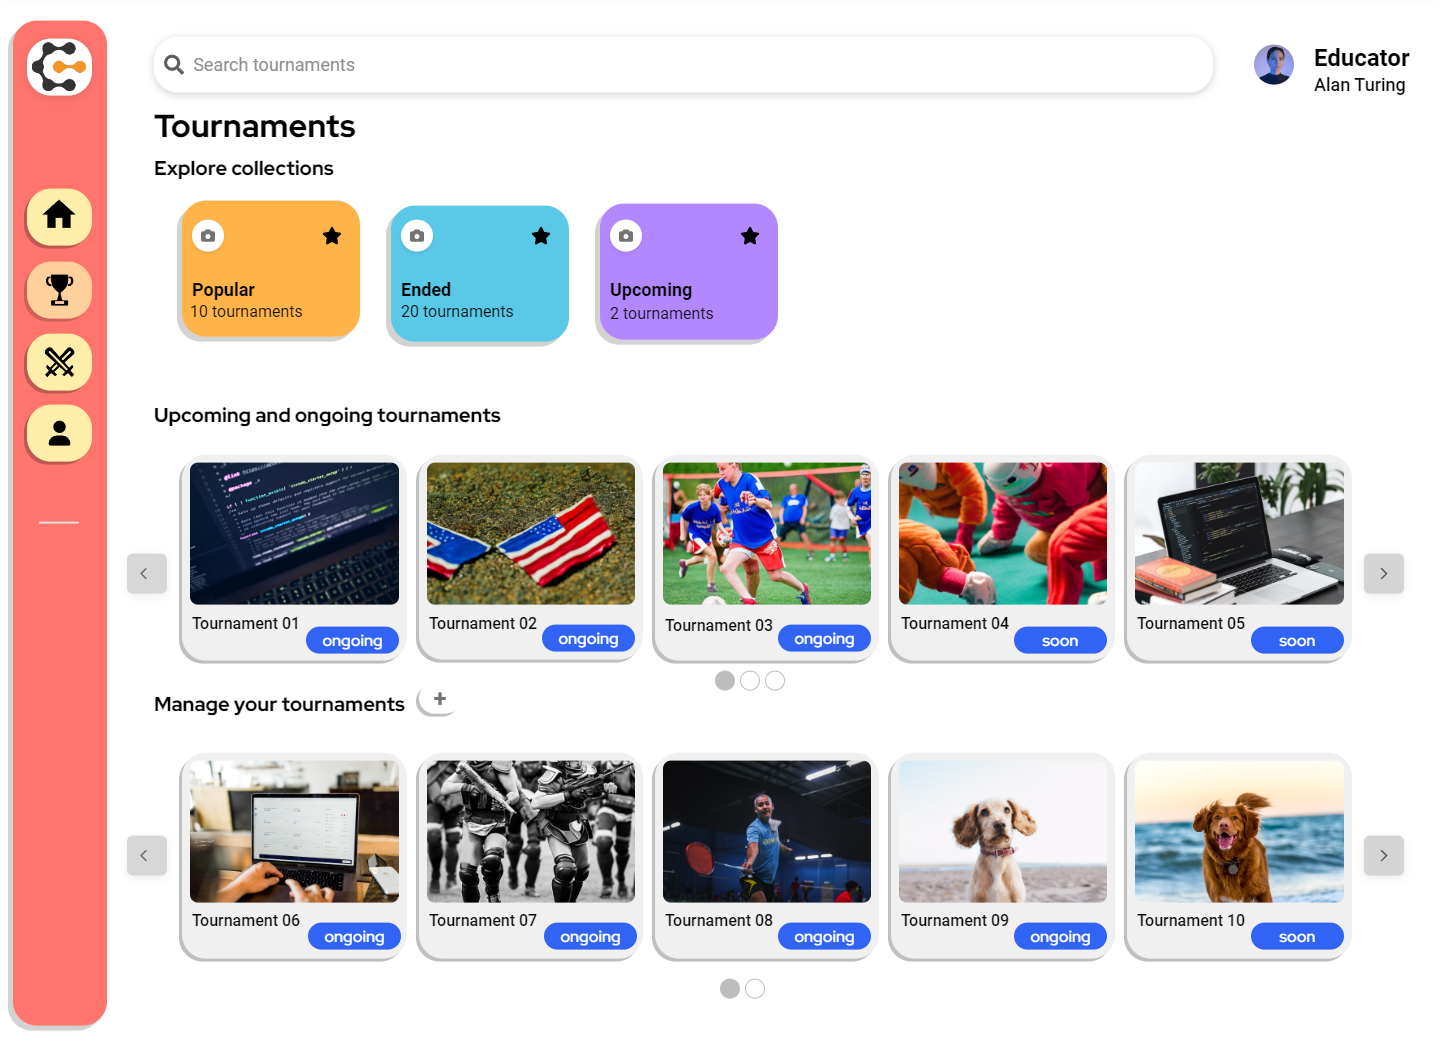
\includegraphics[width=0.8\textwidth]{Mockups/5_educator_tournaments.png}
    \caption{Tournaments page from the perspective of an user logged as educator}
\end{figure}
\begin{figure}[H]
    \centering
    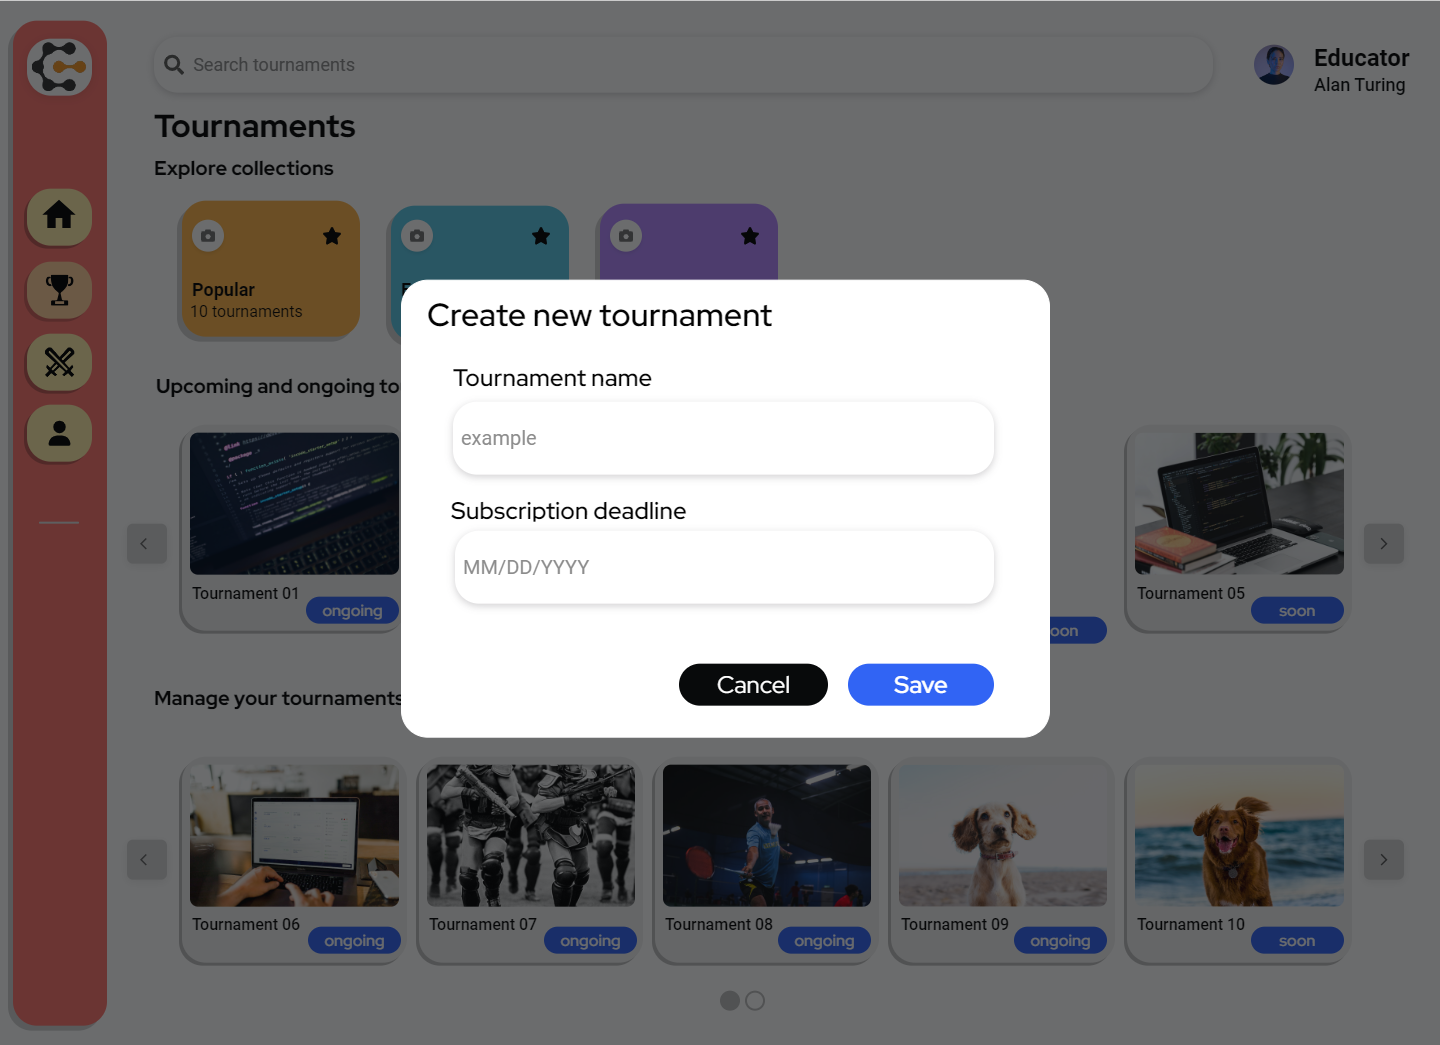
\includegraphics[width=0.8\textwidth]{Mockups/6_educator_create_tournament.png}
    \caption{Page used from educators to create a new tournament}
\end{figure}
The tournament page offers to the educator owning the tournament the possibility to manage it. He will be able to click the "Add collaborator" button to add another educator to the tournament by email address. Moreover, the page offers the "collaborators" tab that can be used to check and manage the list of collaborators. The last tab called "leaderboard" allows the educator to check the ranking of the students enrolled in the tournament. The main tournament page contains the list of all the battles created within the tournament.  By clicking on a specific battle, the educator will be redirected to the battle's page. Most importantly, the educator can create a battle by clicking on "Create battle" button.\\
The student's tournament page will share most of the content, but the options to manage the tournament. The same page, if the tournament is not started yet, offers the possibility to the student to subscribe to the tournament and by default shows a list of partipants. \\
\begin{figure}[H]
    \centering
    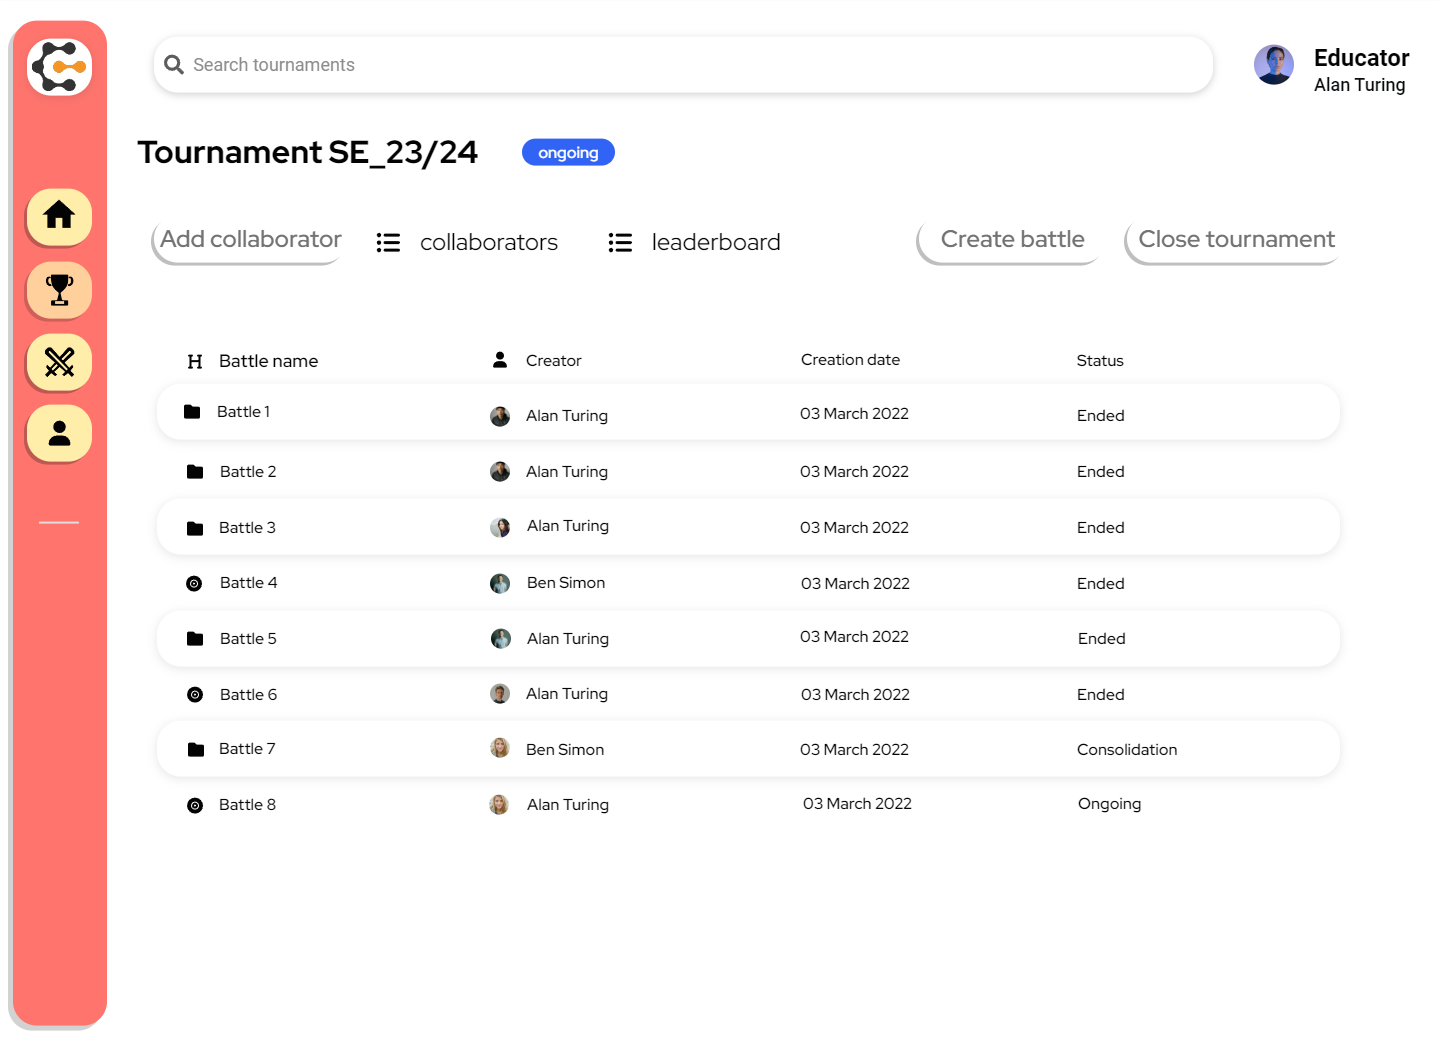
\includegraphics[width=0.8\textwidth]{Mockups/7_educator_manages_tournament.png}
    \caption{Page used from educators to manage the main settings of an ongoing tournament}
\end{figure}
\begin{figure}[H]
    \centering
    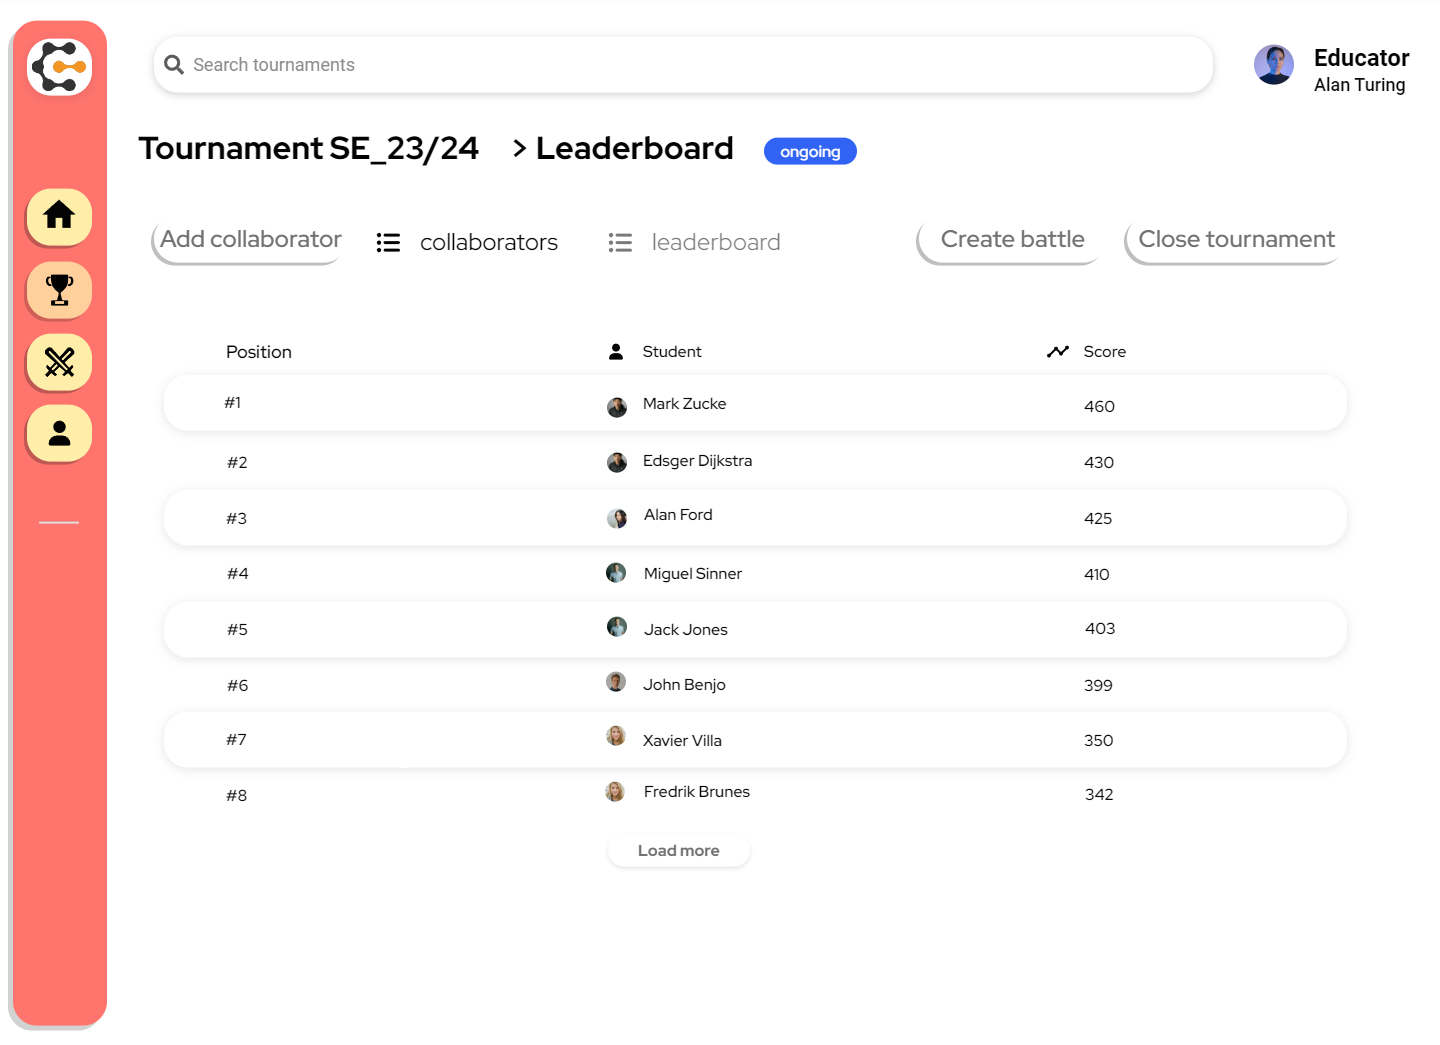
\includegraphics[width=0.8\textwidth]{Mockups/8_educator_tournament_leaderboard.png}
    \caption{"Leaderboard" tab available to both educators and students to check the ranking in tournament}
\end{figure}
\begin{figure}[H]
    \centering
    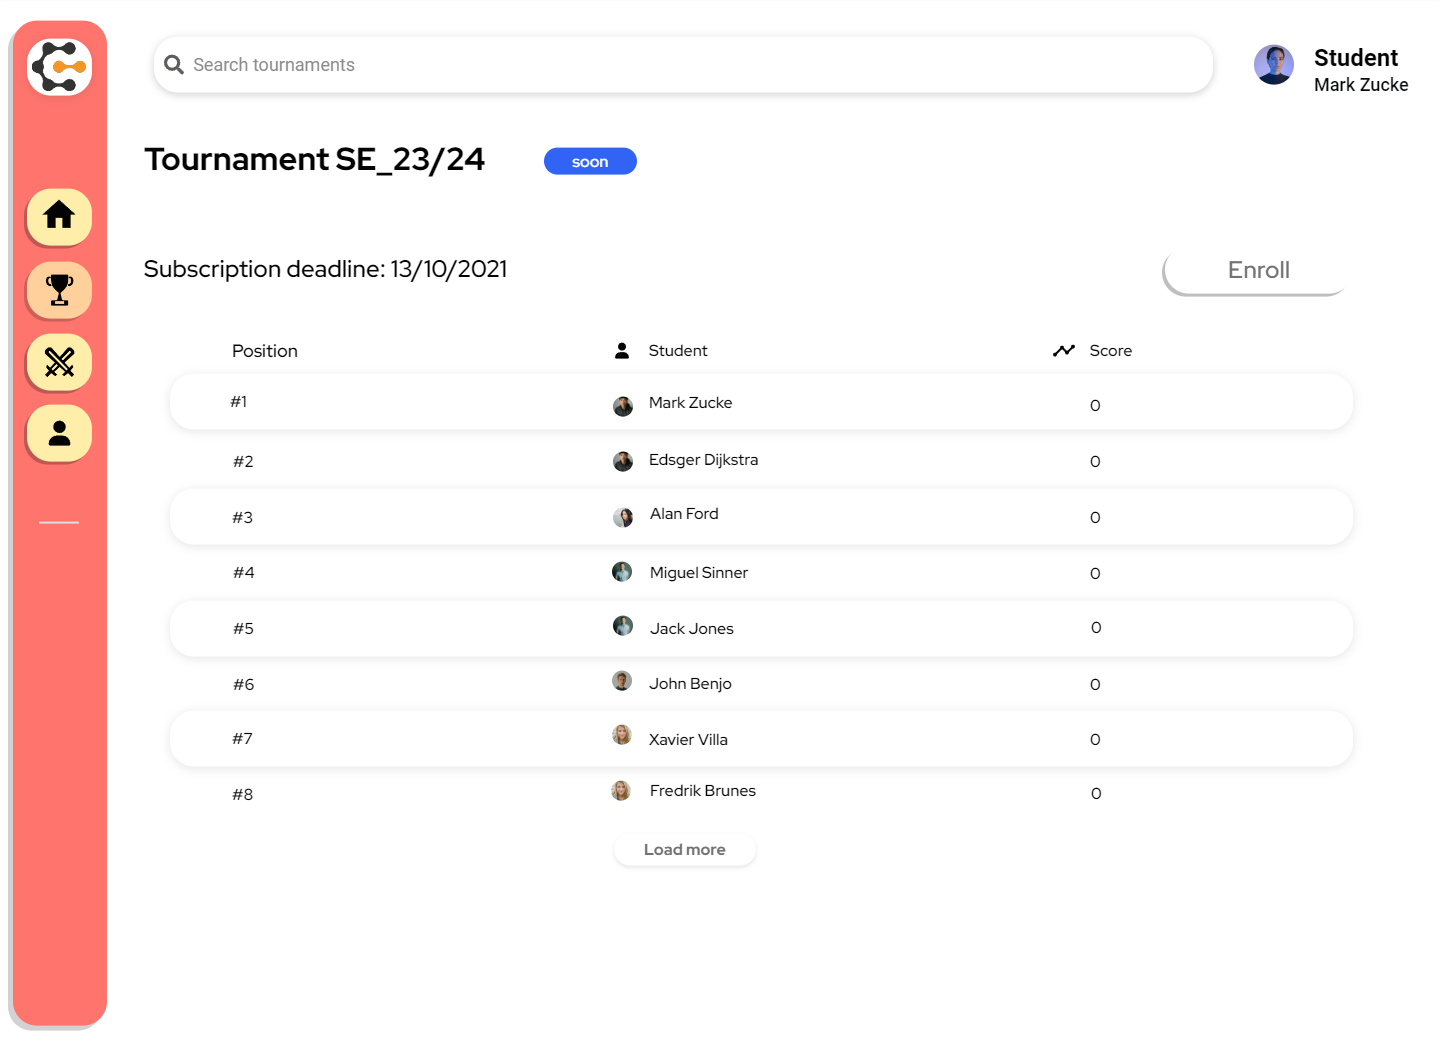
\includegraphics[width=0.8\textwidth]{Mockups/9_student_tournament_subscription.png}
    \caption{Page used from students to subscribe to a tournament}
\end{figure}

\subsection{Battles}
After selecting the option to create a battle, the educator will be redirected to the page used to create a new battle. The page will ask the educator to provide the name of the battle, the description, the deadline for the registration and the deadline for the submission. Moreover, the educator will be able to select the minimum and maximum number of students per group allowed for the battle. The educator will be able to set some information about the battle and to configure the battle settings for the evaluation. He will be required to upload the Code Kata files of the battle, which contain the test cases and the basic template of the project that students will have to complete with their solutions.
\begin{figure}[H]
    \centering
    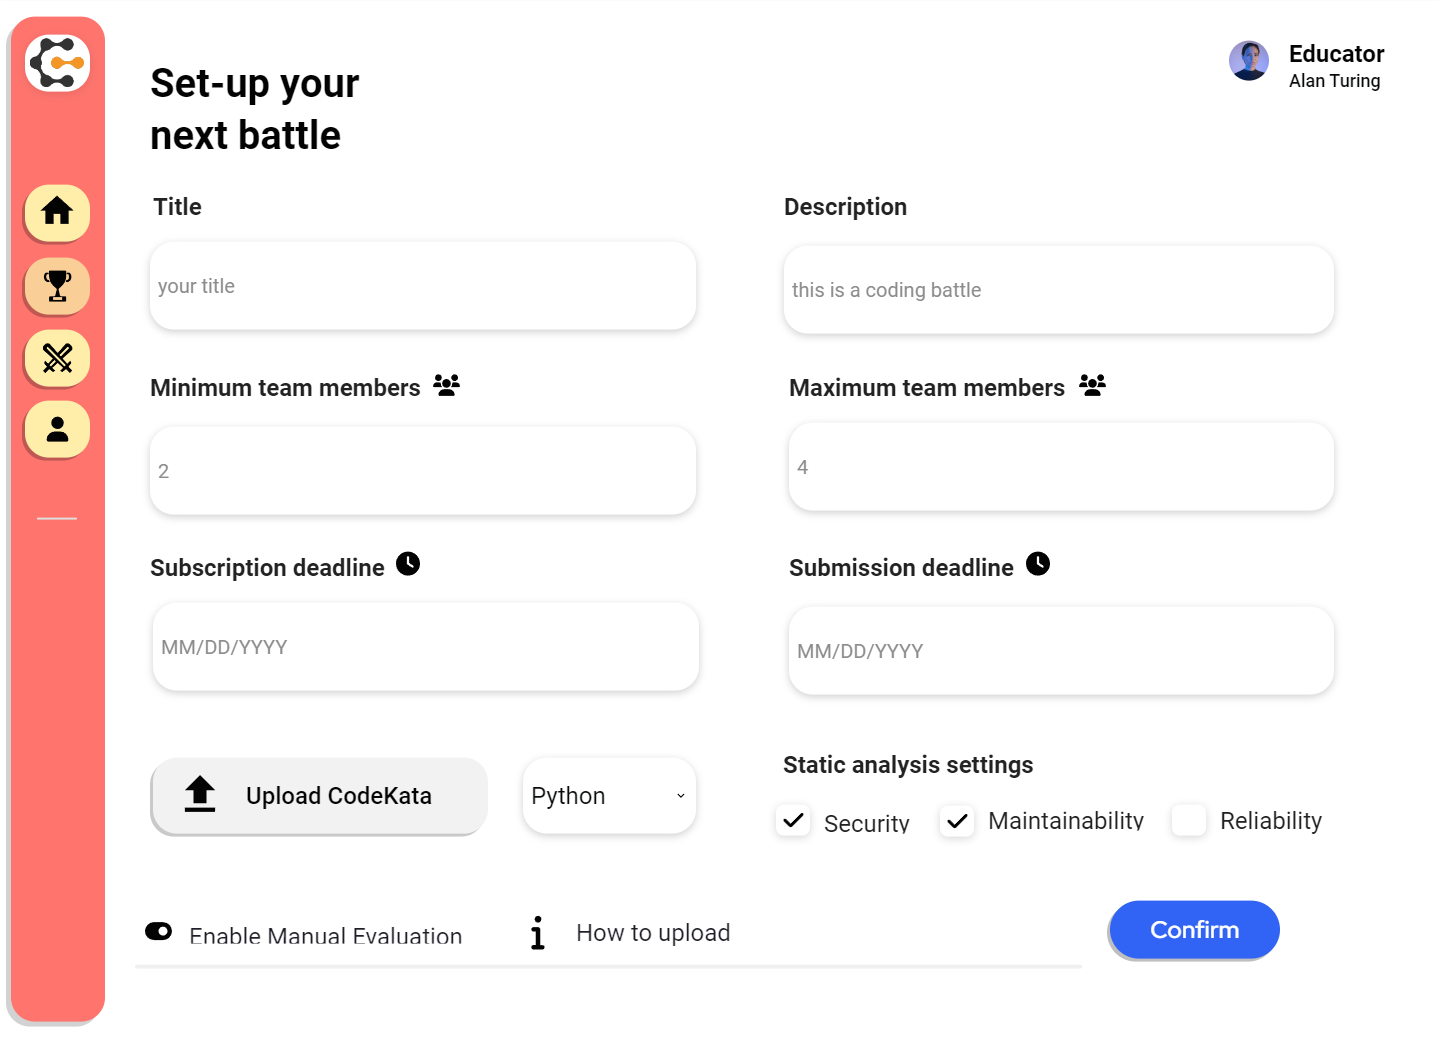
\includegraphics[width=0.8\textwidth]{Mockups/10_educator_create_battle.png}
    \caption{Page used from educators to create a new battle}
\end{figure}
When a battle is in subscription phase, the battle's page will offer to the student the options to subscribe to it by creating a new team or joining an already existing one. If the student decides to create the team, he will be asked to input the name of the team and its privacy setting. Instead, if the student want to join a team, the system will ask him to insert the name of the team (if public) or the invite code (if private). The page will also show the list of all the teams enrolled in the battle, to facilitate the team formation. Teams can be clicked in the leaderboard and a small pop-up with the list of members will be shown.\\
\begin{figure}[H]
    \centering
    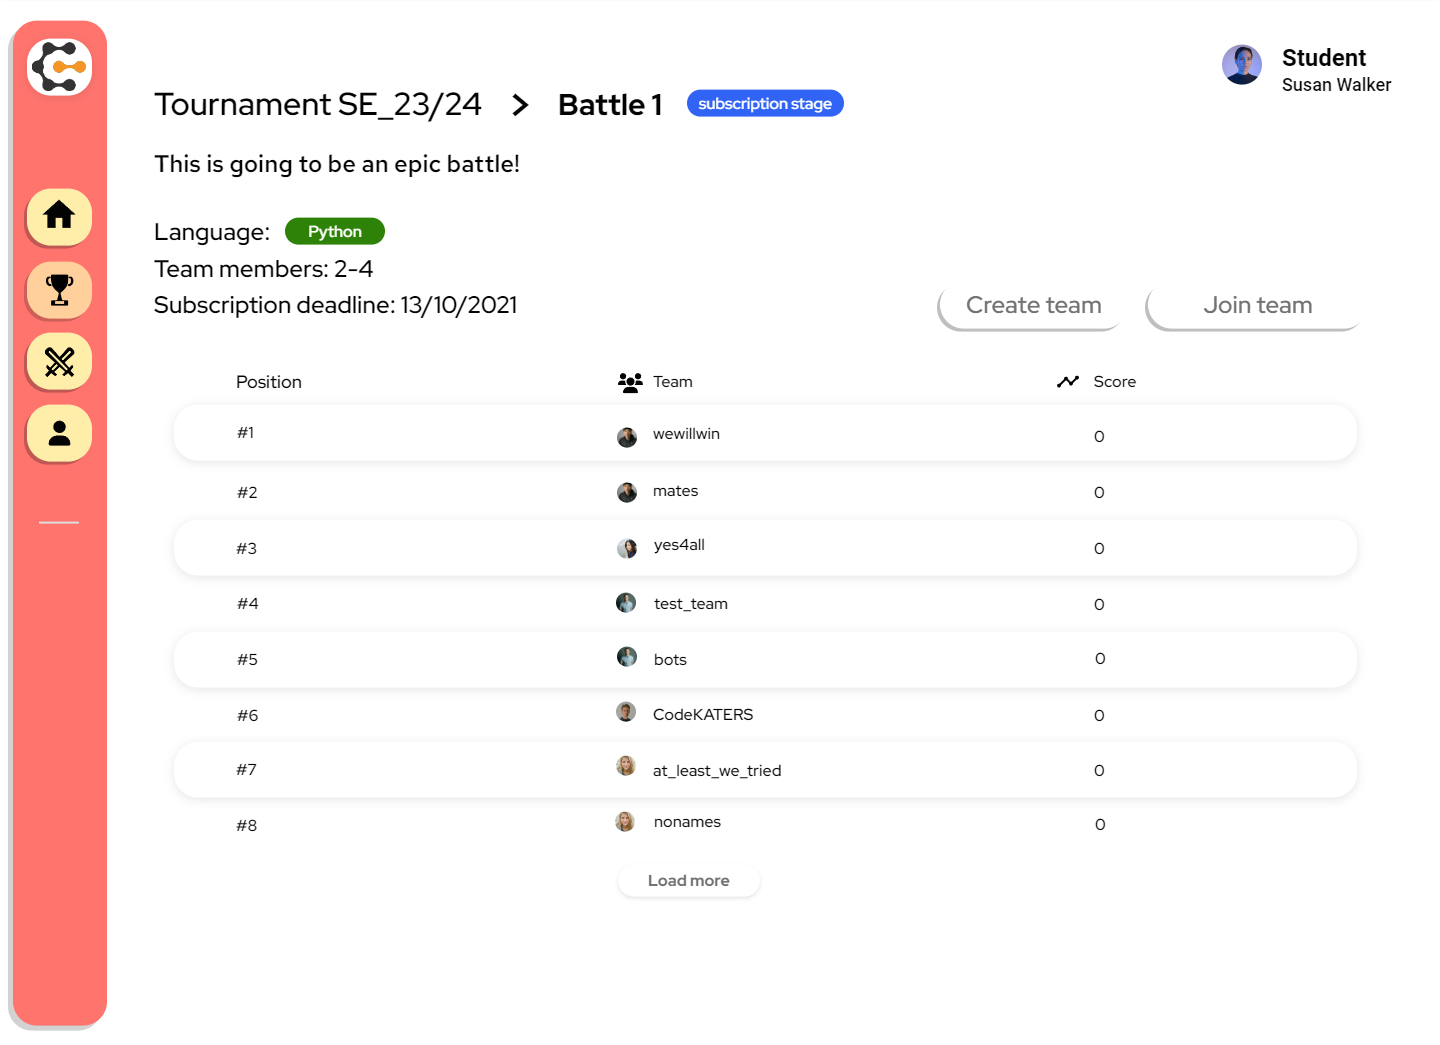
\includegraphics[width=0.8\textwidth]{Mockups/11_student_battle_subscription.png}
    \caption{Page used from students to subscribe to a battle}
\end{figure}
\begin{figure}[H]
    \centering
    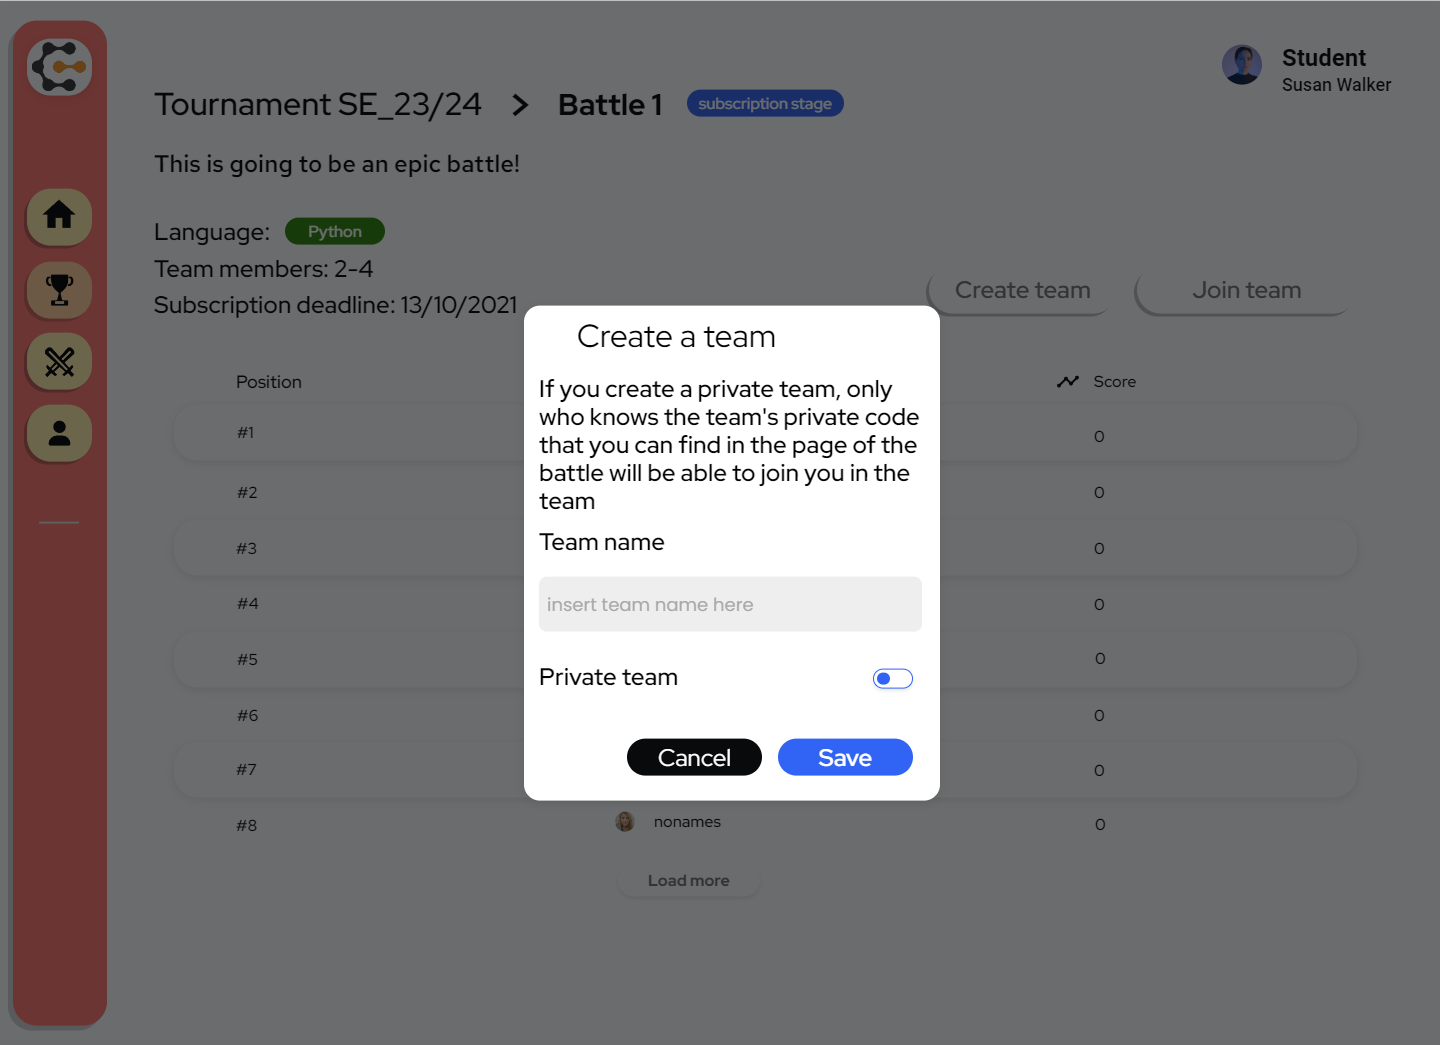
\includegraphics[width=0.8\textwidth]{Mockups/12_student_create_team.png}
    \caption{Page used from students to create a new team}
\end{figure}
\begin{figure}[H]
    \centering
    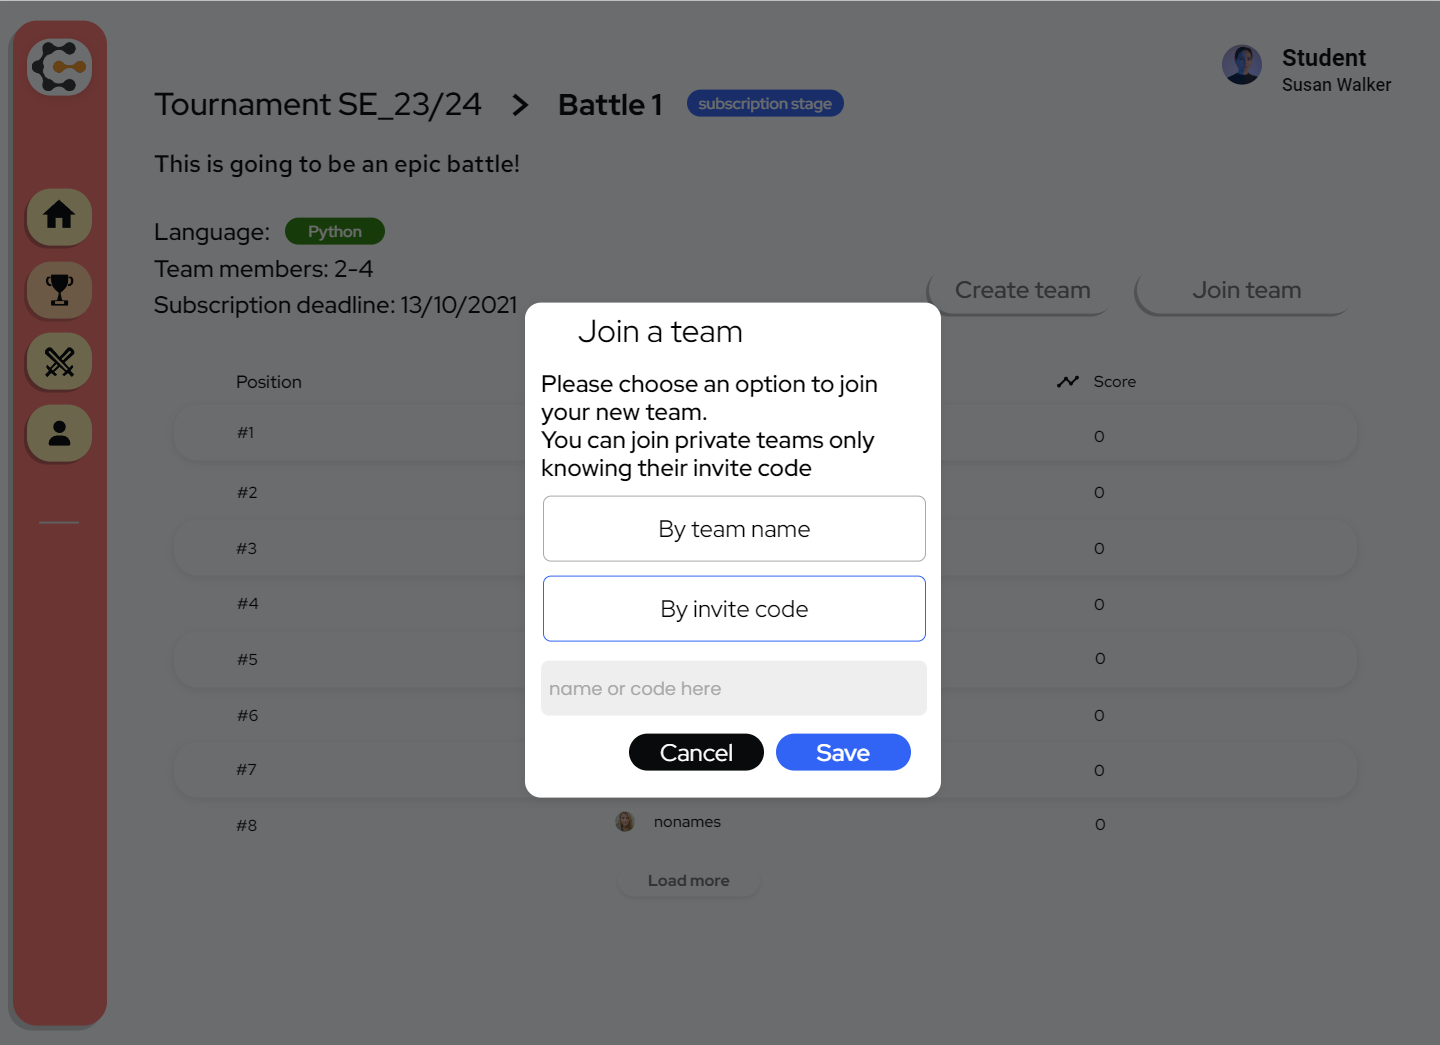
\includegraphics[width=0.8\textwidth]{Mockups/13_student_join_team.png}
    \caption{Page used from students to join a team}
\end{figure}
The page of a battle which is in the submission phase, will show by default the leadeboard of the teams. By clicking on "Your team" button, the student will be able access a section that contains important team settings and the information related to the submissions.\\
In case the manual evaluation is not enabled, this page will have similar content for both educators and students, but the team settings button.\\
\begin{figure}[H]
    \centering
    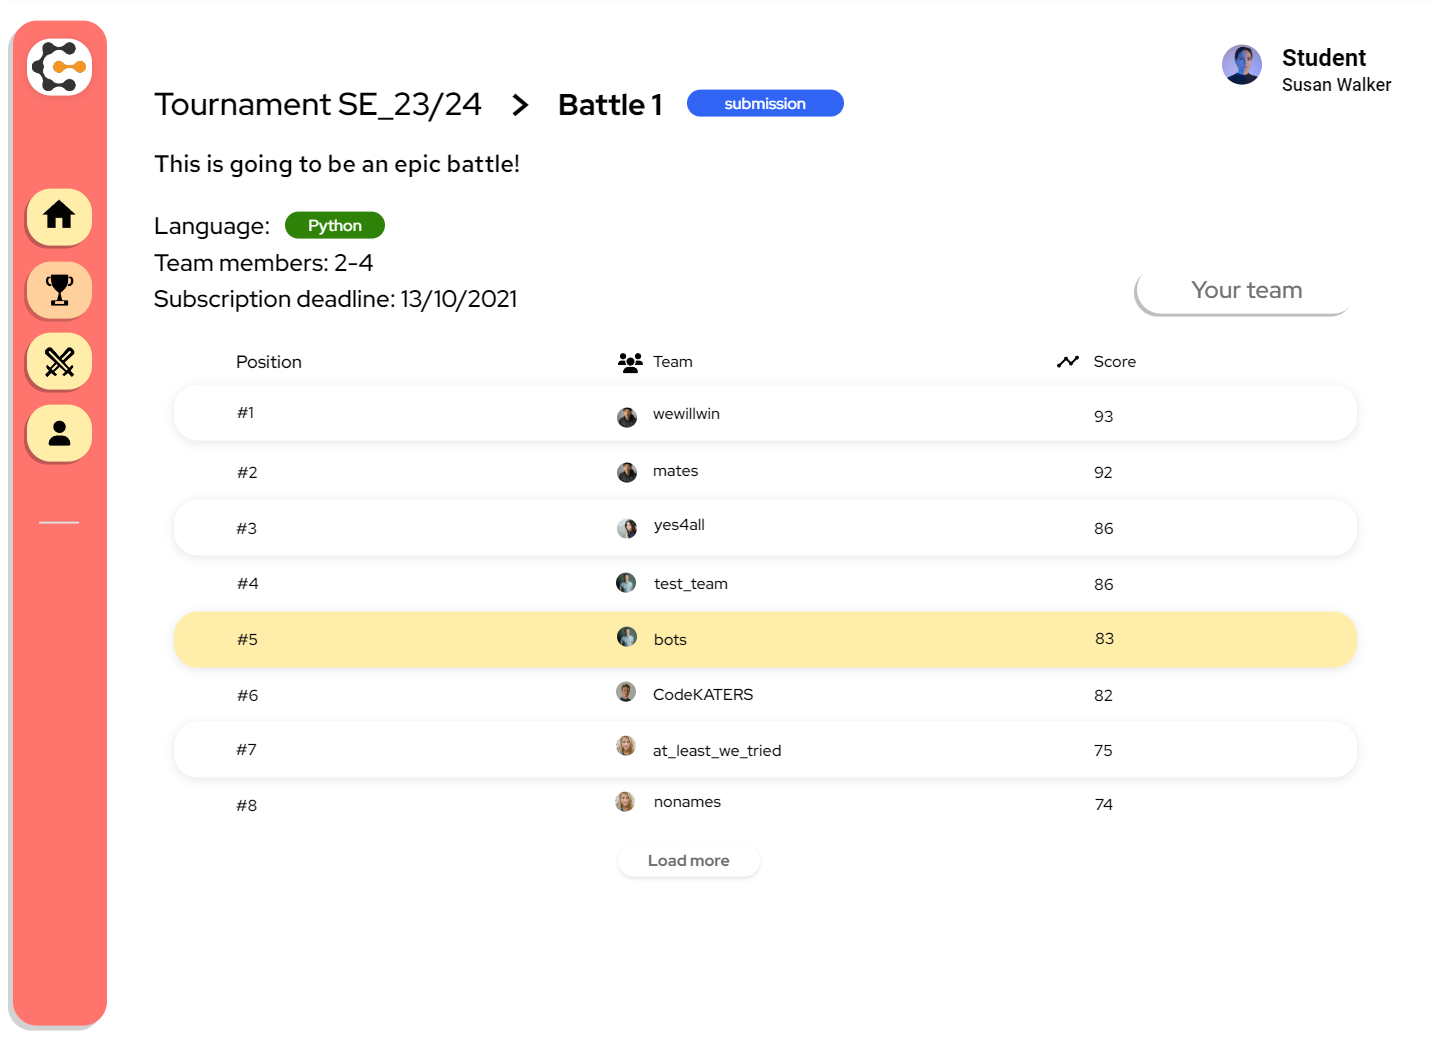
\includegraphics[width=0.8\textwidth]{Mockups/14_student_battle_submission.png}
    \caption{Page used from students when a battle is in submission phase}
\end{figure}
The team page, accessible only to students of team, will contain all important settings needed to properly setup the GitHub repository and evaluation information about the team's last submission. It will show also some statistics about past submissions to facilitate the tracking of the team's performances.
By clicking on "Team members" box, the list of teammates will show up, with related commits count.\\
\begin{figure}[H]
    \centering
    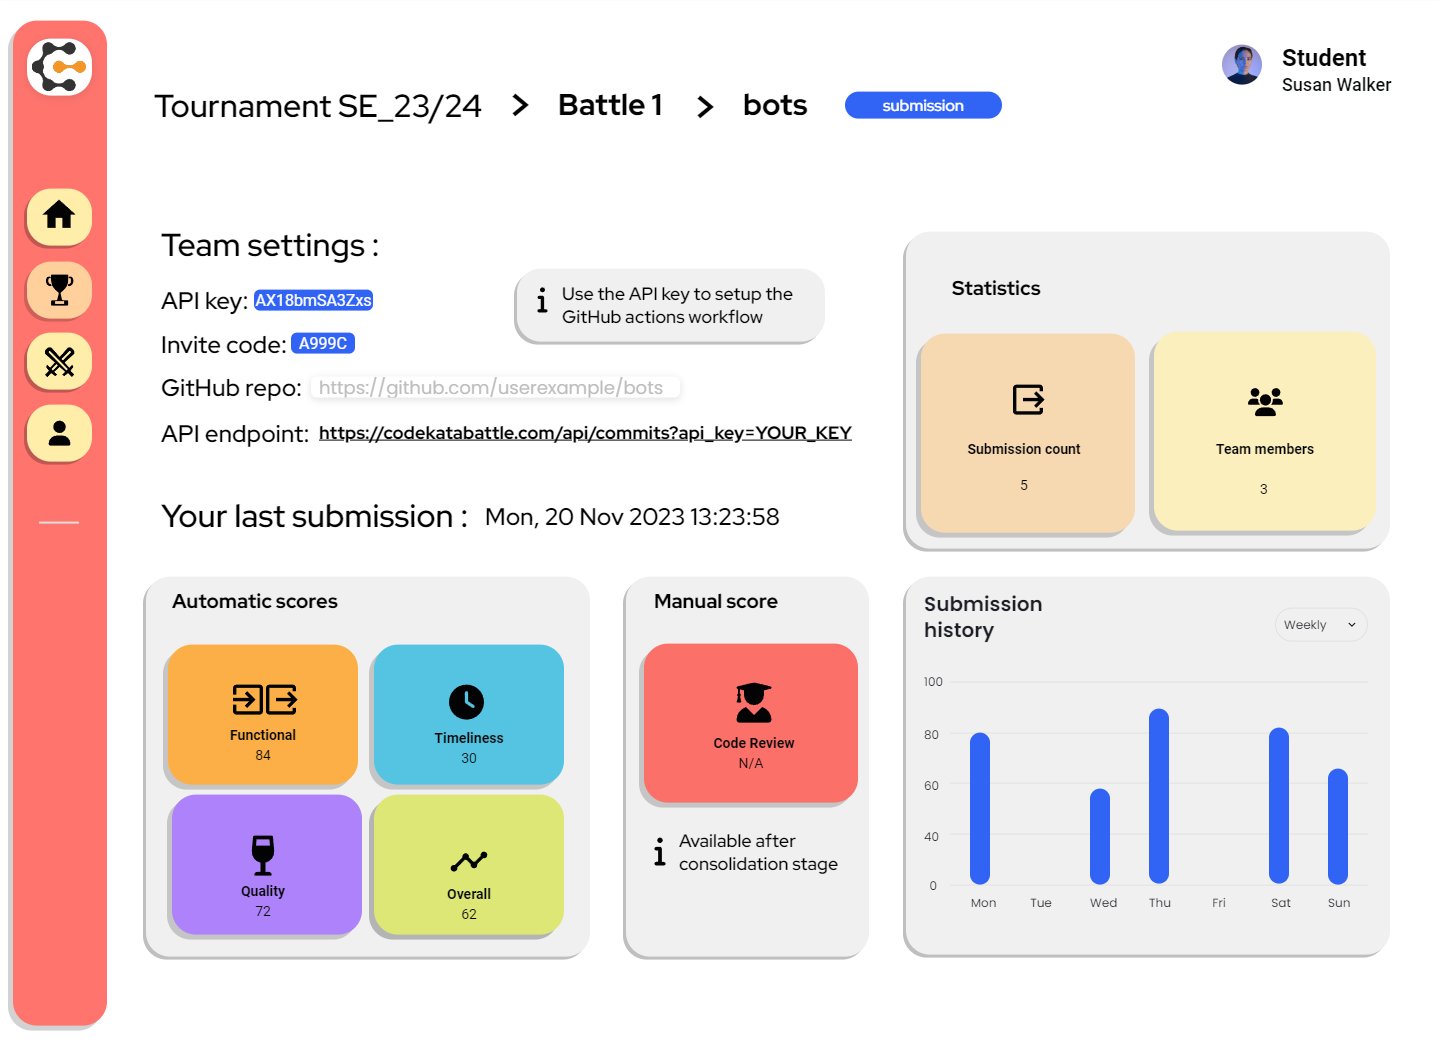
\includegraphics[width=0.8\textwidth]{Mockups/15_student_team.png}
    \caption{Page used from students to manage the settings of their team and to check submissions information}
\end{figure}
    
\subsection{Evaluation}
The battle page, during the optional consolidation stage, will offer a special team leaderboard, with an overview of both manual and automatic scores. By clicking on a specific team, the educator has access to the evaluation page of the team. The page also contains a button to close the consolidation phase once the educator has evaluated all the teams.\\
In the evaluation section, the educator is able to access the GitHub repository of the team to check the code of the last submission. Finally, he is provided with a field to input the manual score.
\begin{figure}[H]
    \centering
    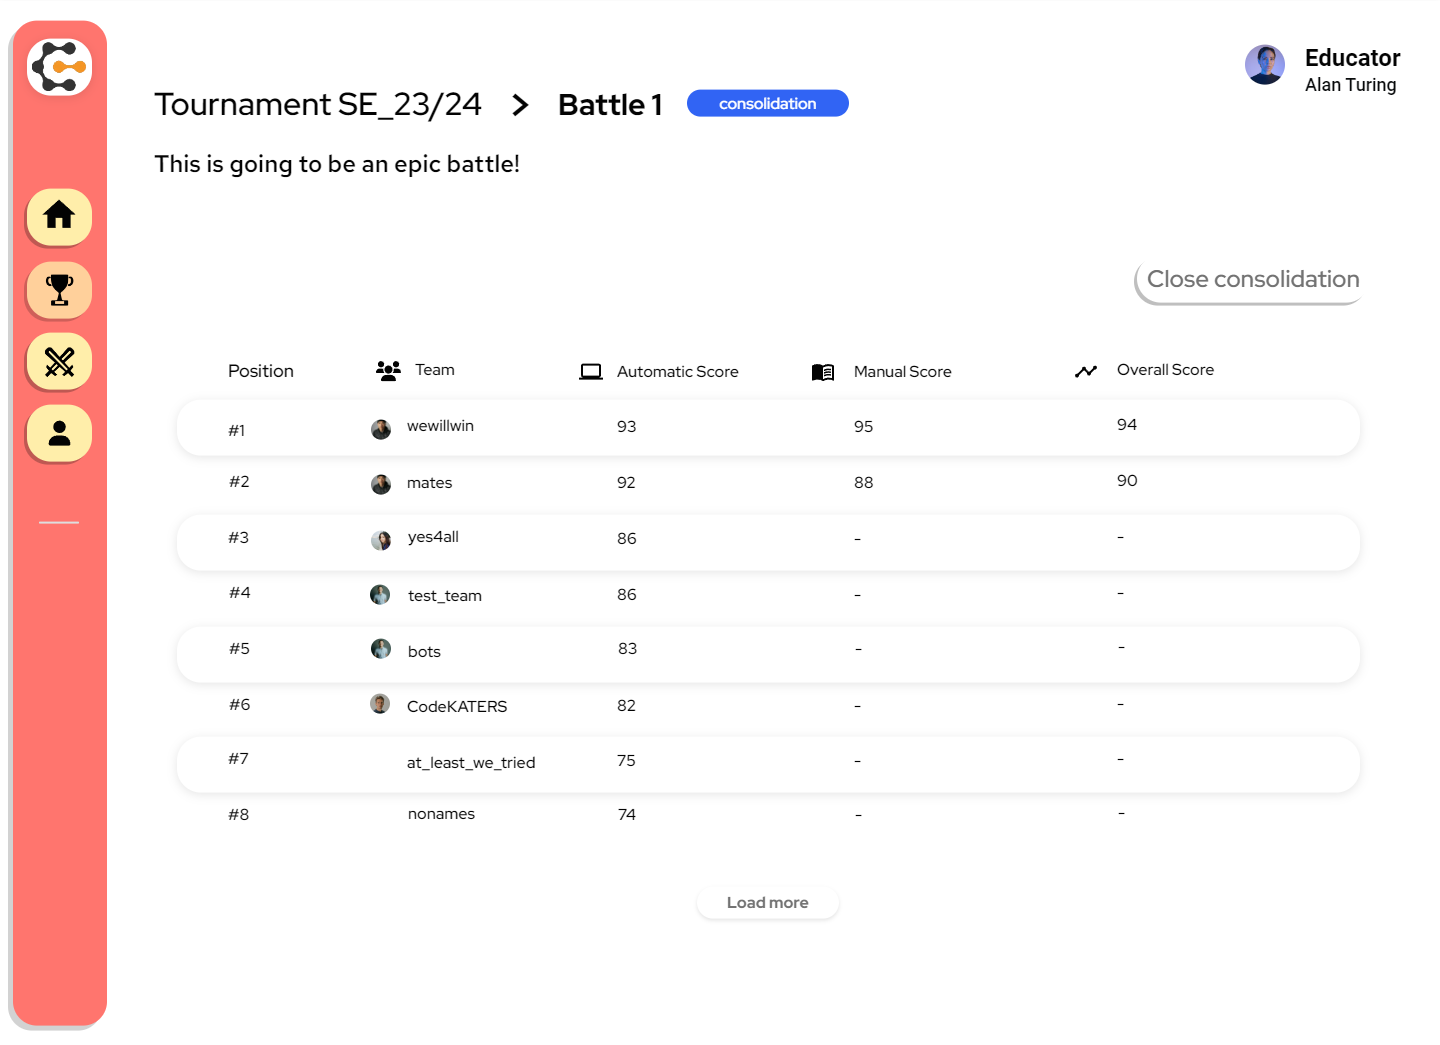
\includegraphics[width=0.8\textwidth]{Mockups/16_educator_battle_consolidation.png}
    \caption{Page used from educators to manage the consolidation stage of a battle}
\end{figure}
\begin{figure}[H]
    \centering
    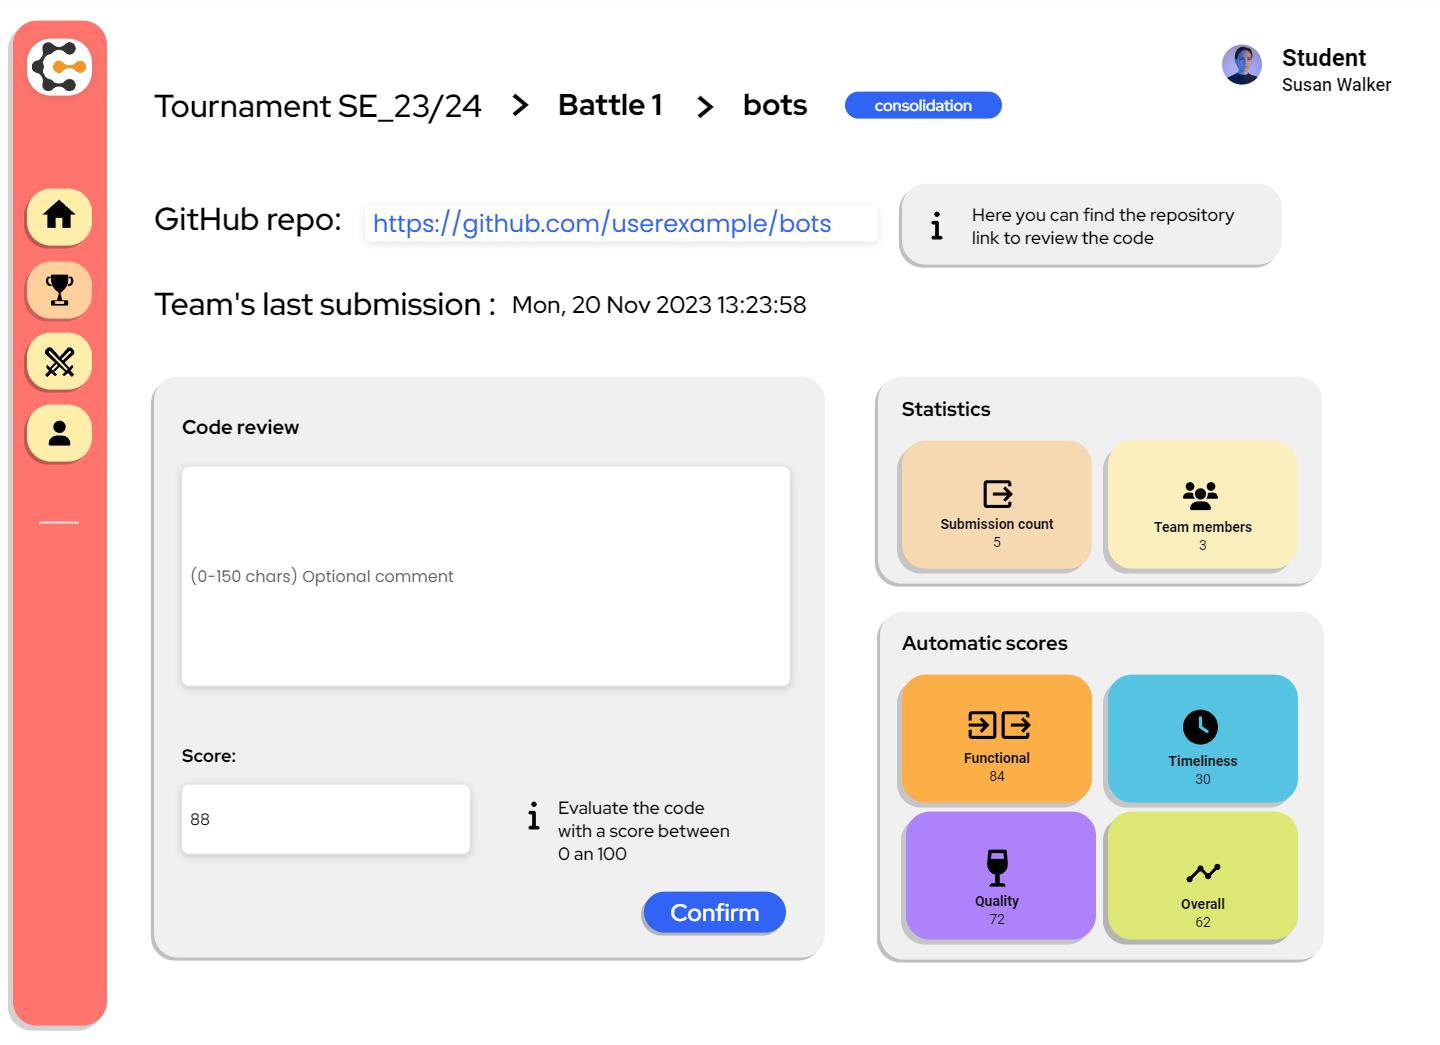
\includegraphics[width=0.8\textwidth]{Mockups/17_educator_manual.png}
    \caption{Page used from educators to manually evaluate a submission}
\end{figure}